\documentclass[tikz,border=10pt]{standalone}
\begin{document}
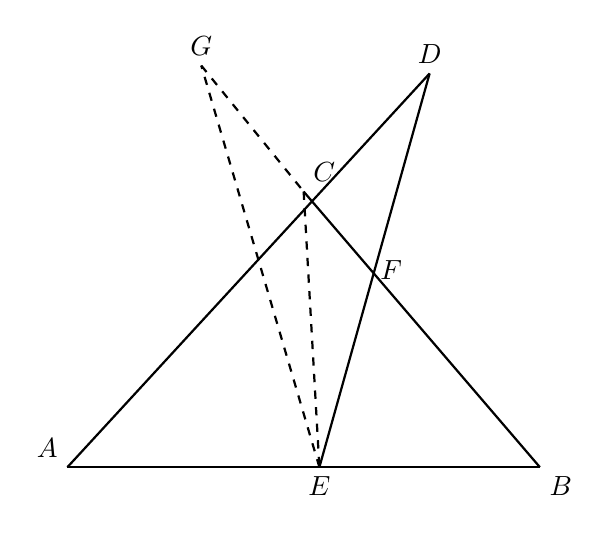
\begin{tikzpicture}[scale=1]
  \coordinate (A) at (0,0);
  \coordinate (B) at (6,0);
  \coordinate (E) at (3.2,0);
  \coordinate (C) at (3,3.5);
  \coordinate (D) at (4.6,5);
  \coordinate (G) at (1.7,5.1);
  \coordinate (F) at (3.85,2.5);

  \draw[thick] (A) -- (B);
  \draw[thick] (A) -- (D);
  \draw[thick] (E) -- (D);
  \draw[thick] (C) -- (B);
  \draw[thick] (E) -- (B);

  \draw[dashed,thick] (C) -- (E);
  \draw[dashed,thick] (E) -- (G);
  \draw[dashed,thick] (G) -- (C);

  \node[above left] at (A) {$A$};
  \node[below right] at (B) {$B$};
  \node[below] at (E) {$E$};
  \node[above right] at (C) {$C$};
  \node[above] at (D) {$D$};
  \node[above] at (G) {$G$};
  \node[right] at (F) {$F$};
\end{tikzpicture}
\end{document}
